\documentclass{standalone}
\usepackage{tikz}
\begin{document}
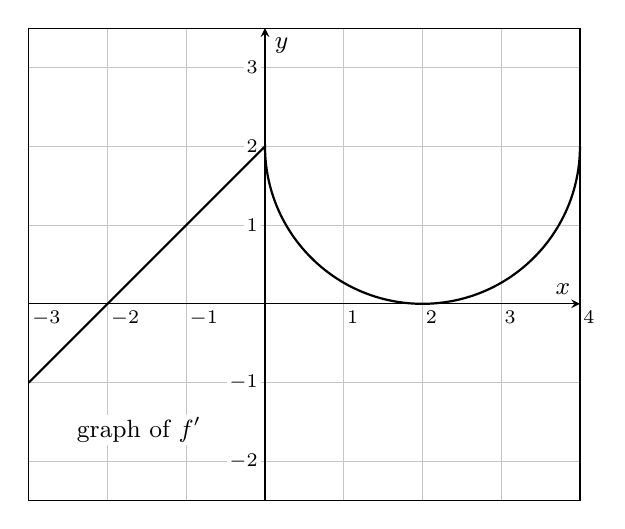
\begin{tikzpicture}[>=stealth, scale=1]
  % Graph of f' on -3 <= x <= 4: a line segment and a semicircle
  %   segment (-3,-1) -- (0,2), i.e. f'(x) = x + 2
  %   lower semicircle centered at (2,2), radius 2, from (0,2) to (4,2)
  \def\xmin{-3}\def\xmax{4}
  \def\ymin{-2.5}\def\ymax{3.5}

  % Grid with frame
  \draw[gray!45] (\xmin,\ymin) grid[step=1] (\xmax,\ymax);
  \draw (\xmin,\ymin) rectangle (\xmax,\ymax);

  % Axes
  \draw[->] (\xmin,0) -- (\xmax,0) node[above left, font=\small] {$x$};
  \draw[->] (0,\ymin) -- (0,\ymax) node[below right, font=\small] {$y$};
  \foreach \x in {-3,-2,-1,1,2,3,4}
    \node[below right, font=\scriptsize, inner sep=1pt] at (\x,-0.05) {$\x$};
  \foreach \y in {-2,-1,1,2,3}
    \node[left, font=\scriptsize, fill=white, inner sep=1pt] at (-0.05,\y) {$\y$};

  % f'
  \draw[thick] (-3,-1) -- (0,2) arc[start angle=180, end angle=360, radius=2];

  % Label
  \node[font=\small, fill=white, inner sep=1pt] at (-1.6,-1.6) {graph of $f'$};
\end{tikzpicture}
\end{document}
